\section{Engine Description}
    The engine concept is taken from the bachelor thesis of \citeauthor{mayer:2023} \cite{mayer:2023}, who is a former member of our student club and contributed to the project. While the chemical reaction in the combustion chamber is designed for operation in flight, the geometry proposed in the bachelor thesis is not optimized for flight, but is intended to ensure the safest possible operation under test conditions. Particularly with regard to the total weight of the engine, adjustments need to be made if the aim is to integrate the propulsion system into a rocket after a successful test on the ground. At this point, it is emphasized once again that the requirements for the engine as presented in this document are not derived from operation in flight, but from horizontal test operation on the ground.
    
    \subsection{Engine Parameters}
        The required engine parameters are listed in table \ref{tab:engine_parameters}. The mass flow rates of fuel and oxidizer are calculated subsequently, according to \citeauthor{mayer:2023}.
        
        \begin{table}[h]
            \centering
            \begin{tabular}{|l|c|c|}
                \hline
                Thrust & $F$ & $750 \siunit{N}$\\
                \hline
                Thrust Chamber Pressure & $p_c$ & $30 \siunit{bar}$\\
                \hline
                Expansion Pressure & $p_e$ & $1 \siunit{bar}$\\
                \hline
                Burn Time & $t_{burn}$ & $5,3\siunit{s}$\\
                \hline
                Oxidizer &  & Liquid Oxygen\\
                \hline
                Fuel &  & $80\% \siunit{Ethanol and}\,20\%\siunit{Water}$\\
                \hline
            \end{tabular}
            \caption[Required engine parameters]{Required engine parameters \cite[p.\,20]{mayer:2023}}
            \label{tab:engine_parameters}
        \end{table}

        A mixing ratio of $\Phi_{Ox/Fu} = 1,1$ is chosen. The specific impulse $I_{sp}$ and the thrust chamber temperature $T_{tc}$ of the reaction are functions of $\Phi_{Ox/Fu}$. The $I_{sp}$ indicates the efficiency of the engine and has a maximum around $\Phi_{Ox/Fu} = 1,5$, however, a lower mixing ratio is chosen to lower the expected temperatures in the engine. With this, a specific impulse of $I_{sp} = 2418,7 \siunit{m/s}$, a thrust chamber temperature of $T_{tc} = 2819,8\siunit{K}$ is calculated \cite[p.\,21]{mayer:2023}. The total mass flow rate is calculated to be:

        \begin{equation}
            \dot{m} = \frac{F}{I_{sp}} = 0.312 \siunit{kg/s}.
        \end{equation}

        The \ac{CEA} package of the \ac{NASA} was used to calculate the expected chamber temperatures and the $I_{sp}$. Mass flow rates of Oxygen and Ethanol can be calculated as:

        \begin{equation}
            \dot{m}_{Eth} = \frac{\dot{m}}{\Phi_{Ox/Fu}+1} = 0.148571\siunit{kg/s}, \text{and}
        \end{equation}

        \begin{equation}
            \dot{m}_{LOX} = \frac{\dot{m}}{1+\frac{1}{\Phi_{Ox/Fu}}} = 0.163429\siunit{kg/s}
        \end{equation}

        Ethanol is mixed with 20\% water to aid cooling. On the fuel side, the total mass flow calculates to be:

        \begin{equation}
            \dot{m}_{\text{Eth/Wat}} = \dot{m}_{Eth} \cdot 1.2 = 0.178286 \siunit{kg/s}.
        \end{equation}

        Fuel and oxidizer are expected to reach the injector plate at $35 \siunit{bars}$ of pressure and $80 \siunit{K}$ or $300 \siunit{K}$, respectively. The densities and dynamic viscosities at these conditions can be obtained from publicly available data sets. The dynamic viscosity of the mixture of ethanol and water can be estimated with the Grunberg-Nissan equation

        \begin{equation}
            \ln{(\eta_{ij})} = \sum_i x_i \cdot \ln{(\eta_i)} + \sum_i \sum_j x_i \cdot x_j \cdot \epsilon_{ij}
        \end{equation}

        
        \begin{table}
            \centering
            \bgroup
            \def\arraystretch{1.5}
            \begin{tabular}{|c||c|c||c|}
                \hline
                 Property & Ethanol & Water & Oxygen\\
                 \hline
                 \hline
                 Mass flow [kg/s]& $0.148571$ & $0.029715$ & $0.163429$\\
                 \hline
                 Density [kg/m$^3$]& $792.383$ & $998.207$ & $1175.58$\\
                 \hline
                 Temperature [K]&\multicolumn{2}{c||}{$300$}& $80$\\
                 \hline
                 Pressure [Pa]& \multicolumn{3}{c|}{$35$}\\
                 \hline
                 Molar mass [kg/kmol]& $46.07$ & $18.015$ & $31.998$\\
                 \hline
                 Molar fraction [1]& $0.5539$ & $0.4461$ & 1\\
                 \hline
            \end{tabular}
            \egroup
            \caption{Thermodynamic properties of fuel and oxidizer at the injector plate.}
            \label{tab:therm.prop.inj.}
        \end{table}

    \subsection{Thrust Chamber and Nozzle Design}


    \subsection{Cooling Concept}


    \subsection{Propellant Injection}


    \subsection{Ignition Concept}
        \subsubsection{Criteria for the Ignition System}
        German law tends to be rather prohibiting, which is why several standard methods to build igniters went out the window for this project. Getting a license, i.e. for the use of black powder, was regarded too much work. %This was since it would be bound to one team member, who would have to be present at all tests and furthermore the time horizon and cost necessary for acquiring one.%
        That means that anything used in the igniter had to be legal and safe to store without special equipment in its assembled state, to transport (i.e. in public transport), to dispose of after testing and to handle without much need for professional safety equipment. \par
        At the moment of cold propellant entering the burn chamber, ignition has to be times precisely for an almost instant ignition to prevent a hard start or even a full explosion of the burn chamber. This means the igniter has to work reliably at a temperature of 89 Kelvin and a pressure of 30 bar (The 30 bar result from the fact that the propellant valves can not be opened incrementally, resulting in no opportunity for a preliminary burn phase.). A burn time of more than one or two second should be part of the system as a safety mechanism, in case the timing does not work as intented. A guidebook by Half Cat Rocketry talks about one second being sufficient for a rocket engine, similar to this one. \cite[63]{mojave_sphinx}\par
        Furthermore a mixed phase state of LOX and ethanol with the ethanol possibly freezing and the LOX not being fully gaseous should not decrease the igniter’s performance. First thermodynamic calculations for the energy needed resulted in about $3 kJ/g$ of propellant. These calculation where rather detailed, compared to what the team saw discussed for comparable rockets, yet with the current funding situation it was concluded that the possibility of a hard start should be minimized, and thus some time spent on calculations would be well invested. The $3 kJ/g$ were calculated by assuming the "worst case" of frozen ethanol coming into contact with the igniter, as the boiling temperature of LOX is below the freezing temperature of ethanol, and then determining the amount of energy necessary to heat the ethanol from -183°C to it's ignition temperature of 425°C: 
      
        
    \begin{flalign}
        %nicht fertig%
        &  c_{p,s}\cdot (159K-89K)+\Delta_{fus}H^\phi + c_{p,l} \cdot (351K-159K) + \Delta_{vap}H^\phi + c_{p,g} \cdot (698K-351K) && \\
        & = 0,111\cfrac{kJ}{molK}\cdot 70 \cdot 4,3 + 4,9 + 0,1124 \cdot 192 + 42,3 + 0.118\cdot 322 &&\\
        &= 140.23 \cfrac{kJ}{mol}&&
    \end{flalign}
    %WOFÜR SIND DIE 4,3???%

    %source: wikipedia data page ethanol%

    % sourve Cp,s, and 4.3??? %    
        
        with $c_{p,s}$, $c_{p,l}$ and $c_{p,g}$ being the solid, liquid and gaseous head capacity of ethanol and $ \Delta_{fus}H^\phi $ and $\Delta_{vap}H^\phi$ being the melting and evaporation enthalpy of ethanol. The temperature differences in brackets equal the degrees Kelvin that the ethanol passes through before reaching the next phase change or the ignition temperature.
        This results in $$\frac{140.23 \quad kJ/mol}{46,68 \quad g/mol}= 3.0 \cfrac{kJ}{g}$$.
        

        
        Of course calculating an energy demand for igniting the fluid has to choose an arbitrary number for the amount of fluid that has to be ignited. Furthermore, LOX being present with the ethanol is not taken into account here.
        \par
        With some questions regarding assembly still open, it is certain that the igniter will be inserted into the engine through the nozzle, due to the small size of the injector plate that does not allow to place it there. This results in the risk of the igniter being blown out by the blast of cold propellants or ejecting out of the burn chamber before ignition. What is more, the igniter would have to be removed from the burn chamber quickly after ignition to not interfere with the burn phase. After a run of the engine, a new igniter should be ready in a short amount of time and show replicable results. 

        \subsubsection{Pyrotechnic Design and Electronics}
        
        The proposed and partially tested ignition powder is thermite consisting of magnesium powder ($< 40µm$) an iron (III) oxide. Some changes to this may occur and the alternative of just using a (modified) solid rocket motor is being evaluated, meaning that the following information regarding thermite could not apply to the final igniter. \par

        In a thermite reaction, a metal oxide reacts vigorously with an elemental metal, oxidizing it and creating a molten mix of metal and metal oxide with a reaction temperature of several thousand Kelvin. For the igniter application, the vigor once activated, but especially the legality of thermite have been deemed critical. Note: The legal knowledge was not obtained by professional counseling, but through personal research and could be incomplete.
        
        \par    
        While safe enough to handle as a team of hobbyists, certain safety protocols need to be followed when using thermite. 
        There is no danger of a spontaneous ignition due to exposure to light or small amounts of heat, however due to the reaction temperature and explosion-like characteristics of the reaction in wet environments, safety measures include:
        \begin{itemize}
            \item Keeping the thermite away from water at all times
            \item Heating storage containers before storing igniters in the to ensure their dryness, plus ensuring a dry testing environment.
            \item Not using the thermite again once wet.
            \item Not using plastic, but instead glass storage containers to avoid static discharge and mixing with something made out of wood/glass
            \item Using basic safety equipment when being close to the igniters during testing. (glasses, gloves)
            \item In case something catches fire, putting it out with dry sand and not CO2, water, foam, etc.
            \item Awareness of the speed of the reaction once started (One batch tends to “go all at once”.).
            \item We could mix the thermite for the igniter at the test site and store the components separately.
        \end{itemize}
        An important factor for the reactivity of metal powders is the fineness of the grain which can be imagined on a spectrum between a coarse grain and harder ignition with more safety and a finer grain with opposite attributes on which an optimum of safety and performance needs to be found. \par

        The type of thermite chosen had to be ignitable by our means, yet not too easily ignited in order to not create a safety hazard. Cuprus oxide for instance was not chosen for the test due to dangers of more spontaneous ignition than in other mixtures. The choice of thermite was in part based on a blog post on “Richard Nakka’s Experimental Rocketry Web Site”\cite{thermite_types}. The author describes the possibility of igniting various magnesium based thermites and many aluminium based mixtures with a mini-bulb igniter. This is realistic for the application in an engine igniter and could be replicated by the team on all occasions for the two mixtures below (albeit using a spark gap instead of a mini-bulb igniter).
        The optimal, stochiometric ratios are 3:1 for red iron oxide with aluminum or 1:2,23 for red iron oxide with magnesium. \par
        The two mixtures would result in the following reactions and energy outputs:
        \begin{equation}
            Fe_2O_3 + 2Al \rightarrow Fe + 2Al_2O_3 , 
            \Delta h = -3.98 \cfrac{kJ}{g}
        \end{equation}

        \begin{equation}
            Fe_2O_3 + 3Mg \rightarrow Fe + 3MgO ,
            \Delta h = -4.21 \cfrac{kJ}{g}
        \end{equation}
   

        \par
        These two types of thermite are ignitable with the following energy: 

        %einbeziehen, dass die ja kalt sind und dabei mehr Energie reinmuss%
        
        
        %das hier gehört nicht hierhin, sondern zur Ethanolrechnung% - Gedeon
        To ensure constantly reaching the needed amount of energy for the ignition process a energy calculation was made. 
        \begin{equation}
            -\frac{d\left[C_{2}H_{5}OH\right]}{dt}=k_{n}\left[C_{2}H_{5}OH\right]^{n}
        \end{equation}
        with
        \begin{equation}
        {n=1,  because}
        \rightarrow 1 \mathrm{C}_2 \mathrm{H}_5 \mathrm{OH}+1 \mathrm{OH} \rightarrow 3 \mathrm{H}_2 \mathrm{O}+2 \mathrm{CO}_2
        \end{equation}
        For $k$ the following equation is given:
        \begin{equation}
        k=A e^{\frac{-E_\alpha}{k T}}
        \end{equation}
        $A$ is given as:
        \begin{equation}
         A = \sigma\sqrt{\frac{8kg\cdot T}{\pi\cdot \mu}} \cdot N_{A}
        \end{equation}
        With a needed Temperature of $T=698 K$, the ignition energy $E_\alpha = 3\frac{kJ}{g}$, the Boltzmann Constant $k_B=1.38 \cdot 10^{-23}\frac{J}{K}$ the reduced mass $m_r = 100 \siunit{g}$ and the collision cross section:
        \begin{equation}
        \sigma=\left(r_A+r_B\right)^2 \cdot \pi 
        \end{equation}
        This resolves in:
        (calculations are not finished yet.)
    \subsubsection{Assembly of the Igniter}

       The chemicals are mixed and inserted into a metal cone or cylinder closed on one side. The exact dimensions still need to be finalised. Initial tests have shown that a length of 6.5 cm is favourable. The diameter of the cylinder must be smaller than the narrowest cross-section of the nozzle. In initial successful tests, an outer diameter of 12 mm was selected. The influence of the wall thickness must also be taken into account. 
       
       Finally, the exposed cable ends are inserted into the open side of the sleeve. This must also be attached to a (wooden) rod that is held in the combustion chamber. Furthermore, the wires leading to and from the opening must also be attached to the rod. \par
        
        \subsubsection{Integration into the engine and test stand}

        To add the ignition system to the test cell, the rod needs to be attached to the ceiling or the sidewalls of a container. This could be managed with ropes or more robust and permanent solutions. Since the wires from the ignition system must be connected safely to the electrical system of the test cell, the latter option would be more realistic. In this approach all reaction products and parts of the wires would be ejected through the nozzle after the ignition. It was contemplated, whether the reaction products would harm the ablative cooling material of the engine in any way, creating combustion instabilities, but due to the high probability of any product getting thrown out of the engine upon combustion that potential damage was disregarded. Another open question is at which point in the process the ignition system is added to the test cell because of the venting of the valves. \par

        The spacial limitations are first, that the nozzle throat diameter is 14,7mm and secondly, the length from the start of the nozzle to the injector plate which is 217,62mm. Igniter positioning in the engine with regards to these measurements is to be tested further, once a test stand is built. \par
        The vessel of the igniter should be conducive to a timed burn with a duration that is long enough to account for timing mistakes.
        To be removed from the engine upon (successful) ignition, the igniter either has to burn fully or eject out of the nozzle. This is still subject to testing. Any igniter would have to resist the gas pressure of about 35bar at the injector from opening the valves, but would have to break away upon ignition.        
        A fully burning igniter would have to be fixated in the burn chamber in a casing that still withstands the opening pressure of the valves. Different ideas for this have been collected, yet the high pressure from opening the fluid valves seems to be a challenge for such a design. \par
        
        With this in mind and an expected higher replicability, an ejecting cartridge is being developed. The cartridge would be fixated on a wooden stick, stuck into the nozzle and fixed to the Engine with some flammable but stable structure, like certain plastics. If testing at a test stand proves that a simple stick is not usable for the setup, further development will take place, but for now, leaning on the use of a similar design by Copenhagen Suborbitals for a much bigger engine, this rather crude design choice stands.\par
        
         \begin{figure}
            \centering
            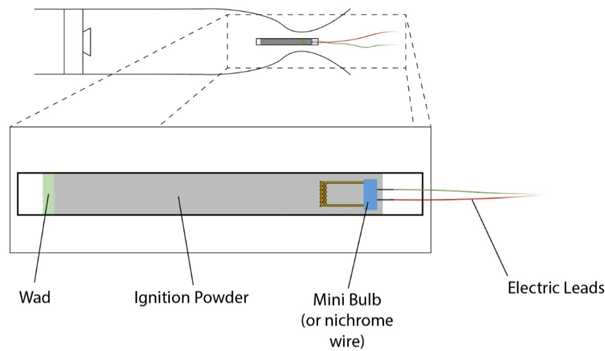
\includegraphics[width=0.6\linewidth]{figures/Sketch of ejecting igniter in engine.png}
            \caption{Sketch for an ejecting igniter within the engine, with an exemplary exploding bridgewire}
            \label{fig:ejecting igniter with engine}
        \end{figure}


        \subsubsection{Validation}
        Several tests of possible designs have been conducted in the past months with some promising results and many lessons learned.\par
        
        When it comes to empirically validating the system, measuring the igniters temperature (i.e. with an IR sensor) was regarded too complicated of a task for such a test and not pursued. So far, the same decision has been made regarding a test of the potential energy output with a bomb-calorimeter. Instead, the team documented the test results with a camera and went for some basic energy output calculations (see above). 
        Another test that might not be necessary with a thermite igniter is a test in something with the volume of the actual engine, as the performance should not be different in environments with different volumes, as there is no gaseous reaction product and the oxygen needed is supplied by the thermite itself.
        %Kommentar: Der letzte Satz könnte falsch sein, wenn man beachtet, dass die gasförmigen Produkte der Treibstoffverbrennung den Druck und die Igniterperformance erhöhen.%
        Instead, the ingiter performance was reviewed mainly by film to determine start time and burn time.\par

        On the first date (July 2024), a setup for cotton-assisted spark ignition from a rocketry handbook was tested. Although helping to get a feeling for the electronics involved, it was only recommended for gaseous oxygen and was limited in terms of energy output. \par

        The second test (08/01/2024) was the first thermite test and was successful in triggering a quickly reacting mixture that was putting out a large amount of heat. Two reaction mixtures were tested. The first was an Ironoxide-Aluminium mixture (2,77g:0,87g), which was stuffed into a paper straw with the cables leading into it from one side and the other side open. The best result in this configuration was provided by rolling the mixture into a cigarette rolling paper. It was ignited by the spark within about two seconds and burned for several seconds along the paper without spreading too much. The reaction temperature had to be reasonably high, due to the small pearls of molten AlO3 forming along the burned paper.  
        The second mixture was an Ironoxide-Magnesium mixture (2,33g:1,12g; 3,41g:1,6g), which was placed into a 5 cm steel tube. One end was taped with the cable ends from the transformer being stuck through the tape while the other end remained open. Additionally, there was a fiercer reaction achieved with addition of small Magnesium pieces of a bigger size than the once used for the thermite. Generally, the tests in this configuration were successful but some problems occurred, which were partially solved in the last takes of this test-campaign. The first problem was that the ignition took place on the opposite side of the igniter opening, resulting in unburnt material being thrown out of the opening and without getting ignited. Secondly sometimes the cables were not positioned with the right distance between cable ends so that no spark could form. What is more, the general assembly of the electronics was suboptimal. 

        The objective of the third test (09/26/2024) was to validate new cable assemblies, work on the exact timing of ignition, check the composition of the chemicals again and try out a new design for the igniter casing. For the latter, the team tested a conical shaped casing with holes in the sidewalls for distribution of the flame which worked out quite good. The preferred mixture was again Ironoxide-Magnesium mixture (3,55g:1,6g). With the cables fixed trough tape, the spark was more reliable but the system still needed improvement. On one take, the igniter was set off 1,0s after the first spark and burned for 1,08s which are promising but not perfect numbers. 

        For future tests the following ideas could be implemented: 
        \begin{itemize}
            \item First, it would be good to verify the performance of the igniter in cold conditions. This could be achieved by testing it, inserted in liquid nitrogen, which is close to the actual burn chamber temperature in the test stand upon ignition. This will have to be coordinated with a lab that has liquid nitrogen. Before that, an ice bath could be worth looking trying as well. 
            \item Secondly, the team needs to decide for a final design of the igniter casing
            \item The chemical composition of the igniter could be enhanced with several things if necessary and legal. Sulphur is cheap and lowers the activation energy of the thermite substantially. Bariumsulphate is used in perchlorate-igniters to contain and concentrate the flame which could be useful to us and is cheap to buy as well. Nitrocellulose Laqueur could be used as a binder and is used by many hobbyists. 
            \item After the team has secured access to LOX, it could also be verified that the igniter does not behave unexpectedly with LOX, though that is not expected to be an issue. This would be important information for test stand safety.
            \item pastly, the igniter should not damage the injector.



        \end{itemize}

        
    
        